% % % % % % % % % % % % % % % % % % % % % % % % % % % % % % % % % % % % 
% 
% FS-Vorlage											Stand: 30.01.12
%
% Formelsammlungsvorlage von Emanuel Regnath und Martin Zellner	
% Bietet verschiedene Abkürzungen und Befehle	
%
% % % % % % % % % % % % % % % % % % % % % % % % % % % % % % % % % % % % 


% Dokumenteinstellungen
% ======================================================================

% Dokumentklasse (Schriftgröße 6, DIN A4, Artikel)
\documentclass[6pt,a4paper]{scrartcl}
%\documentclass[5pt,a4paper]{scrartcl} %USE IN CASE OF EMERGENCY  geschafft! emergency not needed

% Pakete laden
\usepackage[utf8]{inputenc}		% Zeichenkodierung: UTF-8 (für Umlaute)   
\usepackage[german]{babel}		% Deutsche Sprache
\usepackage{amsmath}			% erlaubt mathematische Formeln
\usepackage{amssymb}			% Verschiedene Symbole
\usepackage{esint}				% erweiterte Integralsymbole
\usepackage{multicol}			% ermöglicht Seitenspalten  
\usepackage{booktabs}			% bessere Tabellenlinien
\usepackage{enumitem}			% bessere Listen
\usepackage{graphicx}			% Zum Bilder einfügen benötigt
\usepackage{pbox}				%Intelligent parbox: \pbox{maximum width}{blabalbalb \\ blabal}
\usepackage{accents}			% Für eigene Ableitungspunkte benötigt
\usepackage{undertilde}
\usepackage{trfsigns}			% Laplace und Fourier
\usepackage{scrtime}
\usepackage{parskip} 			%Verhindert das einrücken am Zeilenanfang
\usepackage{titlesec}
\usepackage{tabularx}


% .:: Seitenlayout und Ränder
% ======================================================================
\usepackage{geometry}
\geometry{a4paper,landscape, left=6mm,right=6mm, top=0mm, bottom=3mm,includeheadfoot} 


% .:: Kopf- und Fußzeile
% ======================================================================
\usepackage{fancyhdr}
\pagestyle{fancy}
\fancyhf{}

   \fancyfoot[C]{von Emanuel Regnath und Martin Zellner - Mail: \emph{info@latex4ei.de}}
   \renewcommand{\headrulewidth}{0.0pt} %obere Linie ausblenden
   \renewcommand{\footrulewidth}{0.1pt} %obere Linie ausblenden

   \fancyfoot[R]{Stand: \today \ um \thistime \ Uhr \qquad \thepage}
   \fancyfoot[L]{Homepage: www.latex4ei.de -- Fehler bitte \emph{sofort} melden.}
	
% Schriftart SANS für bessere Lesbarkeit bei kleiner Schrift
\renewcommand{\familydefault}{\sfdefault} 
% Array- und Tabellenabstände vergrößern
\renewcommand{\arraystretch}{1.2}

% Eigene Befehle
\newcommand{\iset}[2]{\ensuremath{\bigl\{ \bigl. #1 \, \bigr| \, #2 \bigr\}}}	%intensional set
\newcommand{\eset}[1]{\ensuremath{\bigl\{#1\bigr\}}}							%extensional set
\newcommand{\enbrace}[1]{\ensuremath{\bigl\(#1\bigr\)}}							%große Klammern
\newcommand{\norm}[1]{\ensuremath{\|#1\|}}										%Norm
\newcommand{\abs}[1]{\ensuremath{\left\vert#1\right\vert}} 						%Betrag
\newcommand{\mat}[1]{\ensuremath{\begin{bmatrix} #1 \end{bmatrix}}}				%Matrix
\newcommand{\ma}[1]{\ensuremath{\utilde{\boldsymbol {#1}}}}						%Matrixsymbol
\newcommand{\vect}[1]{\ensuremath{\begin{pmatrix} #1 \end{pmatrix}}}			%Vektor
\newcommand{\mvect}[1]{\ensuremath{\left. \begin{matrix} #1 \end{matrix}  \right]}} %Matrixvektor
\newcommand{\gk}[1]{\ensuremath{\left\lfloor#1\right\rfloor}} 					%Gaußklammer
\newcommand{\sprod}[2]{\ensuremath{\left\langle #1, #2 \right\rangle }}			%Skalarprodukt
\newcommand{\bdot}{\ensuremath{\boldsymbol \cdot}} 								%Dicker Punkt für Skalarprodukt
\newcommand{\svdots}{\ensuremath{\olddot :}}													% small vertical dots




% Befehle sichern
\let\oldvec = \vec
\let\olddot = \dot
\let\oldlaplace = \laplace
\let\oldfourier = \fourier

% Überschreibungen
\renewcommand{\vec}[1]{\ensuremath{\underline{\boldsymbol {#1}}}}
\renewcommand{\emph}[1]{\textbf{#1}}
\renewcommand*{\dot}[1]{\accentset{\mbox{\textrm{\large\bfseries .}} }{#1}}
\renewcommand*{\ddot}[1]{\accentset{\mbox{\textrm{\large\bfseries .\hspace{-0.25ex}.}}}{#1}}
\renewcommand{\i}{\ensuremath{\mathrm{j}}}										%imaginäre Einheit

% Abkürzungen
\newcommand{\ul}[1]{\ensuremath{\underline{#1}}}								%Untersteichen
\newcommand{\ol}[1]{\ensuremath{\overline{#1}}}									%Überstreichen
\newcommand{\Ra}[0]{\ensuremath{\Rightarrow}}									%Rightarrow
\newcommand{\ra}[0]{\ensuremath{\rightarrow}} 									%Rightarrow
\newcommand{\bs}[1]{\ensuremath{\boldsymbol{#1}}}								%Fett und kursiv im mathmode
\newcommand{\diff}{\ensuremath{\ \mathrm d}}									%delta
\newcommand{\grad}{\ensuremath{\mathrm{grad}\,}}								%Gradient
\renewcommand{\div}{\ensuremath{\mathrm{div}\,}}								%Divergenz
\newcommand{\rot}{\ensuremath{\mathrm{rot}\,}}									%Rotation
\newcommand{\Sp}{\ensuremath{\mathrm{Sp}\,}}									%Spur
\newcommand{\alg}{\ensuremath{\mathrm{alg}}}									%alg. Vielfachheit
\newcommand{\geo}{\ensuremath{\mathrm{geo}}}									%geo. Vielfachheit
\newcommand{\ggT}{\ensuremath{\mathrm{ggT\,}}}									%ggT
\newcommand{\sgn}{\ensuremath{\mathrm{sgn\,}}}									%Signum
\newcommand{\heavi}{\ensuremath{\mathrm{u}}}									%Heaviside Funktion
%\newcommand{\e}{e}																%Eulersche Zahl
\renewcommand{\laplace}{\ \; \oldlaplace \ \;}
\renewcommand{\fourier}{\laplace}

	% Für Mengen
	\newcommand{\N}{\ensuremath{\mathbb N}}
	\newcommand{\R}{\ensuremath{\mathbb R}}
	\newcommand{\C}{\ensuremath{\mathbb C}}
	\newcommand{\Z}{\ensuremath{\mathbb Z}}
	\newcommand{\K}{\ensuremath{\mathbb K}}
	

% .:: Überschriften anpassen
% ======================================================================

%\titleformat{ command }[ shape ]{ format }{ label }{ sep }{ before-code }[ after-code ]
\titleformat{\section}{\Large \bfseries}{\thesection .}{0.5em}{}[\hrule \hrule ]
\titleformat{\subsection}{\large \bfseries}{\thesubsection .}{0.3em}{}[ ]

%\titlespacing{Überschriftart}{keine Ahnung}{Abstand oberhalb}{Abstand unterhalb}
\titlespacing{\section}{0em}{1.0em}{0.1em}
\titlespacing{\subsection}{0em}{0.2em}{-0.4em}
\titlespacing{\subsubsection}{0em}{0em}{-0.5em}



% Dokumentbeginn
% ======================================================================
\begin{document}


% Aufteilung in Spalten
\vspace{-4mm}
\begin{multicols}{4}
	\vspace{-20mm}{
	\parbox{2.3cm}{
		
\includegraphics[height=1.4cm]{../img/Logo.pdf}		
	}
	\parbox{4cm}{
		\emph{\Large{Höhere Mathematik 3}}
	}}
\vspace{-4mm} % Man muss optimieren wos nur geht ;)
% -------------------------------------------
% | 		Mathematik 3					|
% ~~~~~~~~~~~~~~~~~~~~~~~~~~~~~~~~~~~~~~~~~~~
%=======================================================================

\section{Nützliches Wissen $e^{\i x} = \cos (x) + \i \cdot \sin(x)$}
\subsubsection{sinh, cosh \quad $\cosh^2(x)  \bs - \sinh^2(x) = 1$}
$\sinh x = \frac{1}{2}(e^x -e^{-x}) \qquad \quad \operatorname{arsinh}\ x:= \ln\left(x+\sqrt{x^2+1}\right) \\
\cosh x  = \frac{1}{2}(e^x +e^{-x}) \qquad \quad \operatorname{arcosh}\ x:= \ln\left(x+\sqrt{x^2-1}\right)$

\begin{tabular}{ll}
	Additionstheoreme &	Stammfunktionen \\
	$\cosh x \,\; + \sinh x \,\,= e^{x}$ & $\int \sinh x \, dx = \cosh x + C$\\
	$\sinh({\rm arcosh}(x)) = \sqrt{x^2 - 1}$ & $\int \cosh x \, dx = \sinh x + C $\\
	$\cosh({\rm arsinh}(x)) = \sqrt{x^2 + 1}$ 
\end{tabular}
\subsubsection{sin, cos \quad $\sin^2(x) \bs + \cos^2(x) = 1$}
$\begin{array}{c|c|c|c|c|c|c|c|c}
x & 0 & \pi / 6 & \pi / 4 & \pi / 3 & \pi / 2 & \pi & \frac{3}{2}\pi & 2 \pi \\ \hline
\sin & 0 & \frac{1}{2} & \frac{1}{\sqrt{2}} & \frac{\sqrt 3}{2} & 1 & 0 & -1 & 0 \\
\cos & 1 & \frac{\sqrt 3}{2} & \frac{1}{\sqrt 2} & \frac{1}{2} & 0 & -1 & 0 & 1 \\     
\tan & 0 & \frac{\sqrt{3}}{3}&	1				 &	\sqrt{3} & \infty & 0 & - \infty & 0\\
\end{array}$ 
\begin{tabular}{l  l} 
	Additionstheoreme &  Stammfunktionen\\
 	$\cos (x - \frac{\pi}{2}) = \sin x$ & $\int x \cos(x) \diff x = \cos(x) + x \sin(x)$\\
 	
 	 $\sin (x + \frac{\pi}{2}) = \cos x$ & $\int x \sin(x) \diff x = \sin(x) - x \cos(x)$\\
 	
 	$\sin 2x = 2 \sin x \cos x $  & $\int \sin^2(x) \diff x = \frac12 \bigl(x - \sin(x)\cos(x) \bigr)$\\
     
 	$\cos 2x = 2\cos^2 x - 1$  & $\int \cos^2(x) \diff x = \frac12 \bigl(x + \sin(x)\cos(x) \bigr)$\\

 	$\sin(x) = \tan(x)\cos(x)$ & $\int \cos(x)\sin(x) = -\frac12 \cos^2(x)$ \\
\end{tabular}

$\sin x = \frac{1}{2\i} ( e^{\i x} - e^{- \i x})$ \qquad $\cos x = \frac{1}{2}( e^{\i x} + e^{- \i x})$\\
$a^x = e^{x \ln a} \qquad \quad \log_a x = \frac{\ln x}{\ln a} \qquad \log(1) = 0$

\subsection{Wichtige Integrale:}
\begin{itemize}\itemsep-3pt
\item Partielle Integration: $\int uv'=uv-\int u'v$
\item Substitution: $\int f(\underbrace {g(x)}_{t}) \underbrace {g'(x)\,\mathrm dx}_{\mathrm dt}=\int f(t)\, \mathrm dt$
\end{itemize}

\everymath{\displaystyle}	% Formeln ab hier groß Schreiben
\begin{math}\renewcommand{\arraystretch}{1.8}
\begin{array}{c|c|c}
F(x) & f(x) & f'(x) \\ \hline 
\frac{1}{q+1}x^{q+1} & x^q & qx^{q-1} \\
\frac{2\sqrt{x^3}}{3} & \sqrt{x} & \frac{1}{2\sqrt{x}}\\
x\ln(x) -x & \ln(x) & \textstyle \frac{1}{x}\\
\frac{a^x}{\ln(a)} & a^x & a^x \ln(a) \\
-\cos(x) & \sin(x) & \cos(x)\\
-\ln |\cos(x)| & \tan(x) & \frac{1}{\cos^2(x)} \\
\ln |\sin(x)| & \cot(x) & \frac{-1}{\sin^2(x)} \\
x\arcsin (x)+\sqrt{1-x^2} & \arcsin(x) & \frac{1}{\sqrt{1-x^2}}\\
x\arccos (x)-\sqrt{1-x^2} & \arccos(x) & -\frac{1}{\sqrt{1-x^2}}\\
x\arctan (x)-\frac{1}{2} \ln \left| 1+ x^2 \right| & \arctan (x) & \frac{1}{1+x^2} \\
e^{(x)} (x-1) & x \cdot e^{(x)} & e^x(x+1)\\
\frac{1}{2} \Bigl(\sqrt{x^2 + 1} x + \sinh^{-1} (x)\Bigr) & \sqrt{1+x^2} & \frac{x}{\sqrt{x^2+1}}
\end{array}
\end{math}
\everymath{\textstyle}
$\int e^{at} \sin(bt) \diff t = e^{at} \frac{a \sin(bt) + b \cos(bt)}{a^2 + b^2}$\\
$\int t \sin(bt) \diff t = \frac{1}{b^2} (\sin(bt) - b t \cos(bt))$\\
$\int t \cos(bt) \diff t = \frac{1}{b^2} (bt \sin(bt) + \cos(bt))$ \\
$\int t e^{at} \diff t = \frac{at-1}{a^2} e^{at}$ \qquad $\int t^2 e^{at} \diff t = \frac{(ax-1)^2+1}{a^3} e^{at}$\\
% $\int e^{at} \sin(bt) \diff t = e^{at} \frac{a \sin(bt) + b \cos(bt)}{a^2 + b^2}$



\subsection{Determinante von $A\in \mathbb K^{n\times n}$: $\det(A)=|A|$}

 $\det\begin{pmatrix}A&0\\C&D\end{pmatrix}=\det\begin{pmatrix}A&B\\0&D\end{pmatrix}=\det(A)\cdot\det(D)$ \\
Hat $\ma A$ 2 linear abhäng. Zeilen/Spalten $\Rightarrow |A|=0$ \\
Entwicklung. n. $i$ter Zeile: $|A|=\sum\limits_{i=1}^n (-1)^{i+j} \cdot a_{ij} \cdot |A_{ij}|$ \qquad 

	\subsubsection{Eigenwerte $\lambda$ und Eigenvektoren $\vec v$}
	\boxed{\ma A \vec v = \lambda \vec v} \qquad $\det \ma A = \prod \lambda_i$ \qquad $\Sp \ma A = \sum \lambda_i$\\\\
	\emph{Eigenwerte:} $\det(\ma A - \lambda \ma 1) = 0$, Det-Entwickl., Polynom-Div. \\
	%$\Ra$ $\chi_A = (\lambda_1 - \chi)^{\nu_1} \cdot ... \cdot (\lambda_r - \chi)^{\nu_r}$ \quad $\nu_i = \mathrm{alg}(\lambda_i)$\\
	\emph{Eigenvektoren:} $\mathrm{Eig}_A (\lambda_i) = \ker(\ma A - \lambda_i \ma 1) = \vec v_i$\\
	$\ra \dim(\mathrm{Eig}_A (\lambda_i)) = \mathrm{geo}(\lambda_i)$ \quad $\forall i : 1 \le \mathrm{geo}(\lambda_i) \le \mathrm{alg}(\lambda_i)$
	\emph{Hauptvektoren}
	Ein Vektor $\vec v$ heißt Hauptvektor $k$-ter Stufe genau dann wenn:
	$(\ma A - \lambda \ma E)^{k} \vec{v} = \vec{0}$ und $(\ma A - \lambda \ma E)^{k-1} \vec v \not = 0$


\subsection{Reihen}

$\underset{\text{Harmonische Reihe}}{\sum\limits_{n=1}^\infty \frac{1}{n} \ra \infty} \qquad   \underset{\text{Geometrische Reihe}}{\sum\limits_{n=0}^\infty q^n \stackrel{|q|<1}= \frac{1}{1-q}}  \qquad \underset{\text{Exponentialreihe}}{\sum\limits_{n = 0}^{\infty} \frac{z^n}{n!} = e^z}$

\subsection{Vektoroperatoren}
$\grad f = \nabla f$ \qquad $\div \vec f = \nabla^\top \bdot \vec f$ \qquad $\rot \vec f = \nabla \times \vec f$\\
$\Delta f = \div{\grad{f}}$



% ==============================================================================================================
\section{Integralarten}
% ==============================================================================================================
	%Satz von Fubini: Falls die Integralgrenzen von den Integranden unabhängig sind, gilt: $\int\limits^d_c \int\limits^b_a ... \diff x \diff y$ = $\int\limits^b_a \int\limits^d_c ... \diff y \diff x$\\
	
		\subsubsection{Regulärer Bereich}
		$B \subseteq \R^n$ heißt \emph{regulärer Bereich}, wenn
		\begin{itemize}
			\item $B$ abgeschlossen und einfach zusammenhängend
			\item $B$ lässt sich in endlich viele Normalbereiche zerlegen\\
		\end{itemize}				
		
		\subsubsection{Volumen und Oberfläche von Rotationskörpern um $x$-Achse}
		$V = \pi \int_a^b f(x)^2 \mathrm dx$ \qquad \quad $O = 2 \pi \int_a^b f(x) \sqrt{1 + f'(x)^2} \mathrm dx$

		\subsection{Skalares Kurvenintegral}
		\boxed{ \int\limits_\gamma f \ \mathrm ds := \int\limits^b_a f\bigl(\vec \gamma(t)\bigr) \cdot \norm{\vec{\dot \gamma}(t)} \mathrm dt } \quad 
		\pbox{4.0cm}{ SF $f(\vec x)$; $\vec x, \vec \gamma \in \mathbb R^n$\\ $L(\vec \gamma) = \int_\gamma 1 \diff s$}\\
		Gesamtmasse $M = \int\limits_\gamma f \ \mathrm ds = \int\limits^b_a \varrho \bigl(\vec \gamma(t)\bigr) \cdot \norm{\vec{\dot \gamma}(t)} \mathrm dt$\\
		Schwerpunkt $\vec S$: \quad $S_i = \frac{1}{M(\vec \gamma)} \cdot \int\limits_\gamma x_i \varrho \ \mathrm ds$
		
		\subsection{vektorielles Kurvenintegral}
		\boxed{ \int \vec v \bs \cdot \mathrm d\vec s := \int\limits^b_a \vec v \bigl(\vec \gamma(t)\bigr)^\top \bs \cdot \vec{\dot \gamma}(t) \ \mathrm dt } \quad VF $\vec v(\vec x)$; $\vec x, \vec v, \vec \gamma \in \mathbb R^n$
		
		\subsubsection{Fluss durch Kurve}
		Fluss von $\vec{v}$ von (in Durchlaufrichtung gesehen) links nach rechts.\\
		\boxed{\int_{\omega}{\vec{v} \diff \vec{n}} = \int_{\omega}{\vec{v} \cdot \begin{pmatrix}
			0 & 1 \\
			-1 & 0 \\
		\end{pmatrix} \vec{T}(\vec{x}) \diff \vec{s}}}\\\\

	
		\subsection{Gebietsintegrale über Normalbereiche}
		$f:B \subseteq \R^2 \ra \R$ stetig
		
		\subsubsection{Flächenintegrale im $\R^2$}
		\emph{Typ I} $B_{\text{I}}$ regulärer Bereich\\
		$B_{\text{I}} = \left\{\vec{x} \in \R^2 | a \leq x_1 \leq b; g(x_1) \leq x_2 \leq h(x_1)\right\}$\\
		\boxed{\iint_B{f \diff F} = \int_{x_1=a}^b{\int_{x_2=g(x_1)}^{h(x_1)}{f(x_1,x_2) \diff x_2}\diff x_1}}
		
		\emph{Typ II} $B_{\text{II}}$ regulärer Bereich\\
		$B_{\text{II}} = \left\{\vec{x} \in \R^2 | c \leq x_2 \leq d; l(x_2) \leq x_1 \leq r(x_2)\right\}$\\
		\boxed{\iint_B{f \diff F} = \int_{x_2=c}^d{\int_{x_1=l(x_2)}^{r(x_2)}{f(x_1,x_2) \diff x_1} \diff x_2}}
		
		\subsubsection{Volumenintegrale im $\R^3$}
		$V$ regulärer Bereich\\
		$V = \{\vec{x} \in \R^3 \vert a \le x_1 \le b, u(x_1) \le x_2 \le o(x_1), u'(x_1,x_2) \le x_3 < o'(x_1,x_2)\}$\\
		\boxed{ \iiint_V f \diff V = \int\limits_a^{b} \int\limits_{u(x_1)}^{o(x_1)} \int\limits_{u'(x_1,x_2)}^{o'(x_1,x_2)} f(x_1,x_2,x_3) \diff x_3 \diff x_2 \diff x_1}
		
		\subsection{Koordinatentransformationen}
		$D, B \subseteq \R^2$ reguläre Bereiche\\
		$\vec{x}:D \ra B$ mit $\vec{x} = \vec{x}(u_1,u_2) \quad \vec{u} \in D$\\
		$\Ra \iint_B{f(x_1,x_2) \diff F(\vec{x})} = \iint_D{f(\vec{x}(u_1,u_2))\abs{\det J_{\vec{x}}(\vec{u})} \diff F(\vec{u})}$\\
		$J_{\vec{x}} \neq 0$ bis auf Nullmengen
		
		$D, B \subseteq \R^3$ reguläre Bereiche\\
		$\vec{x}:D \ra B$ mit $\vec{x} = \vec{x}(u_1,u_2,u_3) \quad \vec{u} \in D$\\
		$\Ra \iiint_B{f(\vec{x}) \diff V(\vec{x})} = \iiint_D{f(\vec{x}(\vec{u}))\abs{\det J_{\vec{x}}(\vec{u})} \diff V(\vec{u})}$\\
		$J_{\vec{x}} \neq 0$ bis auf Nullmengen
		
		\subsubsection{Koordinatenwechsel}
		$\vec{x}:\vec{u} \in D \ra \vec{x}(\vec{u}) \in B$ orthogonale Transformation\\
		$D, B \subseteq \R^3$\\
		
		$B(\vec{u}) = \begin{pmatrix}
			\vec{e}_{u_1} & \vec{e}_{u_2} & \vec{e}_{u_3}\\
		\end{pmatrix} \quad \vec{e}_{u_i} = \frac{\vec{x}_{u_i}}{\norm{\vec{x}_{u_i}}}$\\
		\boxed{\vec{v}(\vec{x}(\vec{u})) = B(\vec{u}) \vec{V}(\vec{u})}
		
		\emph{Kurvenintegrale}\\
		$\omega(t) \in D$: Kurve im $\vec{u}$-Raum\\
		$\tilde{\vec{\omega}}(t) = \vec{x}(\vec{\omega}(t))$: Zugehörige Kurve im $x$-Raum\\
		
		$\vec{v}(\vec{x}) \cdot \diff \vec{x} = \vec{V}(\vec{u}) \cdot \vect{h_1 \diff u_1 \\ h_2 \diff u_2 \\ h_3 \diff u_3\\} = \vect{h_1 V_1(\vec{u}) \\ h_2 V_2(\vec{u}) \\ h_3 V_3(\vec{u})\\} \cdot \diff \vec{u}$\\
		$\diff \vec{x} = h_1 \vec{e}_{u_1} \diff u_1 + h_2 \vec{e}_{u_2} \diff u_2 + h_3 \vec{e}_{u_3} \diff u_3$\\
		$\diff s(\vec{x}) = \sqrt{h_1^2 \dot{\omega_1}(t)^2 + h_2^2 \dot{\omega_2}(t)^2 + h_3^2 \dot{\omega_3}(t)^2} \diff t$
		
		\emph{Oberflächenintegrale}\\
		$T \subset D$: Fläche im $u$-Bereich\\
		$S \subset B$: Entsprechende Fläche im $x$-Bereich\\
		$S = \vec{x}(T)$; Parametrisierung in D: $(u,w) \in M \mapsto \vec{\phi}(u,w)$
		\begin{gather*}
			\iint_S{\vec{v} \cdot \diff\vec{O}} = \iint_M\left(V_1 h_2 h_3 \frac{\partial(\phi_2,\phi_3)}{\partial(u,w)}\right.\\ \left.+ V_2 h_3 h_1 \frac{\partial(\phi_3,\phi_1)}{\partial(u,w)} + V_3 h_1 h_2 \frac{\partial(\phi_1,\phi_2)}{\partial(u,w)}\right) \diff s \diff t
		\end{gather*}
		\begin{gather*}
			\diff\vec{O}(\vec{x}) = \left[h_2 h_3 \frac{\partial(\phi_2,\phi_3)}{\partial(u,w)}\vec{e}_{u_1}\right.\\ \left. + h_3 h_1 \frac{\partial(\phi_3,\phi_1)}{\partial(u,w)}\vec{e}_{u_2} + h_1 h_2 \frac{\partial(\phi_1,\phi_2)}{\partial(u,w)}\vec{e}_{u_3}\right] \diff s \diff t
		\end{gather*}
		
		\subsection{Integration über Flächen in $\R^3$}
		
		\subsubsection{Parametrisierung}
		Fläche im Zweidimensionalen wird zuerst parametrisiert:\\
		$(u,w) \in M \mapsto \vec{\phi}(u,w) = \vec{x} \in \R^3$
		
		Kreis mit Radius $r$:\\
		$\phi = x^2 + y^2 \le r^2$ \qquad $\partial \phi = \vect{r \cos(t)\\ r \sin(t)}$ \quad $\vec n = \vect{r \cos(t)\\ r \sin(t)}$\\[0.5em]
		Ellipse mit den Halbachsen $a$ und $b$:\\
		$\phi = \frac{x^2}{a^2} + \frac{y^2}{b^2} \le 1$ \qquad $\partial \phi = \vect{ a \cos(t) \\  b \sin(t)}$ \quad $\vec n = \vect{ a \cos(t) \\ b \sin(t)}$
		
		\emph{Eigenschaften der Parametrisierung $\vec{\phi}(u,w)$}
		\begin{itemize}
			\item $x$ flächentreu: $\norm{\vec{\phi}_u \times \vec{\phi}_w} = 1$
			\item $x$ winkeltreu: $\vec{\phi}_u \perp \vec{\phi}_w$ \& $\norm{\vec{\phi}_u} = \norm{\vec{\phi}_w}$
			\item $x$ längentreu: $\vec{\phi}_u \perp \vec{\phi}_w$ \& $\norm{\vec{\phi}_u} = \norm{\vec{\phi}_w} = 1$
		\end{itemize}
		% Torrus mit:\\
%	
%	\begin{tabular}{l|l|l|l}
%		Form & Fläche & Rand & Normalvektor\\ \midrule
%		\pbox{4cm}{ Kreis mit \\ Radius $r$} & $x^2 + y^2 \le r$ & $\bigl( r \cos(t), r \sin(t) \bigr)$ & $ \% $ \\ \midrule
%		\pbox{4cm}{ Ellipse mit den \\ Halbachsen $a$ und $b$} & $\frac{x^2}{a^2} + \frac{y^2}{b^2} \le 1$ & $\bigl( a \cos(t), b \sin(t) \bigr)$ & $\vect{ b \cos(t) \\ a \sin(t) }$ \\ \midrule
%		\pbox{4cm}{ Torus mit \\ Radius $R$ und } & \\
%	\end{tabular}
%
%		Umrechnung Karth. in Polar falls orthogonal:\\
%		$\int\limits_x \int\limits_y f(x,y) \diff y \diff x \ra \int\limits_\phi \int\limits_r f(r \cos (\phi), r \sin(\phi)) \boldsymbol r \diff r \diff \phi$\\
%		Sonst: $\int\limits_x \int\limits_y f(\vec x) \diff x \diff y \ra \int\limits_\varphi \int\limits_r f(\vec x(r, \varphi)) \det \ma J_{\vec x}(r,\varphi) \diff r \diff \varphi$\\		
		
		\subsubsection{Skalares Oberflächenintegral}
		Fläche $\vec \phi: B \subseteq \R^2 \ra \R^3, (u,w) \mapsto \vec \phi(u,w)$ und SF $f$\\
		\boxed{ \iint_{\vec \phi} f \diff O := \iint_B f\bigl(\vec \phi(u,w)\bigr) \cdot \norm{ \vec \phi_u \times \vec \phi_w } \diff u \diff w }
		
		\subsubsection{Vektorielles Oberflächenintegral (Fluss)}
		VF $\vec v:D\subseteq \R^3 \ra \R^3, \vec x \mapsto \vec v(x,y,z)$ und Fläche $\vec \phi(u,w)$ \\
		\boxed{ \iint_{\vec \phi} \vec v \bdot \diff \vec O := \iint_B \vec v\Bigl(\vec \phi(u,w)\Bigr)^\top \bdot \Bigl( \vec \phi_u \times \vec \phi_w \Bigr) \diff u \diff w }
		% Falls eine Stammfunktion zu $\vec v$ existiert, dann ist der Fluss wegunabhängig


% ==============================================================================================================		
\section{Integralsätze}
% ==============================================================================================================

	Ist $B \subseteq \R^2$ Gebiet mit geschlossenem Rand $\partial B = \sum \vec \gamma_i$ mit $\vec \gamma_i \in \mathcal C^1$ 
	und pos. param. (gegen Uhrzeigersinn), dann  gilt $\forall \mathcal C^1$ VF $\vec v$:
	
	\subsection{Divergenzsatz von Grauß für einfache $\partial V = \sum \phi_i$}
	\boxed{ \iiint_V \div \vec v \diff x \diff y \diff z = \oiint_{\partial V} \vec v \bdot \diff \vec O = \sum \iint_{\vec \phi_i} \vec v \bdot \diff \vec O}\\
	$\vec \phi_i$ muss pos. param. sein! ($\vec n = \phi_{iu} \times \phi_{iy}$ nach außen)\\
	\\
	Für Fläche $A$: \boxed{ \iint_A \div \vec v \diff A = \oint_{\partial A} \vec v \Bigl( \vec \gamma(t) \Bigr)^\top \vec n \diff s  }\\
	$\diff s = \norm{ \dot{\vec \gamma}(t) } \diff t$ \qquad $\vec n = \norm{\vec{ \dot \gamma}}^{-1} (\gamma_2, -\gamma_1)^\top$
	
	\subsubsection{Sektorformel zur Flächenberechnung}
	$\omega(t) = \partial B$\\
	\boxed{F(B) = \frac{1}{2} \int_a^b{\omega_1 \dot{\omega_2} - \omega_2 \dot{\omega_1} \diff t}}

	\subsection{Satz von Stokes für doppelpunktfreien $\partial \phi = \sum \gamma_i$}
	\boxed{ \iint_{\vec \phi} \rot \vec v \diff \vec O = \oint_{\partial \vec \phi} \vec v \diff \vec s } \qquad
	\pbox{4.0cm}{Rechte Hand Regel:\\ Flächennormale = Daumen \\ Umlaufrichtung = Finger }\\  %Stetige Deformation		
	
	\subsubsection{Satz von Green}
	\boxed{ \iint_B \frac{\partial v_2}{\partial x} - \frac{\partial v_1}{\partial y} \diff x \diff y = \oint_{\partial B} \vec v \bdot \diff \vec s = \sum\limits_{i=1}^k \int_{\vec \gamma_i} \vec v \bdot \diff s }\\  
	\\
	%Fläche von $B$: $F(B) = \frac12 \oint_{\partial B} \vect{ 0 \\ \gamma_1 } \norm{\dot{\vec \gamma}(t)} \diff t$ \quad $\partial B = \sum \vec \gamma_i$
	
	\subsubsection{Satz von Stokes für ebene Felder}
	$\vec{v}:B \subseteq \R^2 \ra \R^2$ und $\vec{e_3} = \vect{0 \\ 0 \\ 1 \\}$\\
	\boxed{\iint_B{\rot{\vect{\vec{v} \\ 0 \\}} \vec{e_3} \diff F} = \oint_{\partial B}{\vec{v} \diff \vec{x}}}\\\\
	Sind $f,g$ zwei SF, so: $\iiint_B f \Delta g + \nabla f \nabla g \diff V = \iint_{\partial B} f \nabla g \diff \vec O$\\
	für $f=1$: $\iiint_B \Delta g \diff V = \iint_{\partial B} \nabla g \diff \vec O$\\
	
	\subsection{Gradientenfeld}
	$D \subset \R^n$ offen und \emph{einfach zusammenhängend} und $\vec{v}(\vec{x})$ mit $\vec{v}:D \ra \R^n$ $C^1$-Vektorfeld. Wenn
	\begin{itemize}
		\item $\rot \vec{v} = 0$ \emph{oder}
		\item $J_{\vec{v}}(\vec{x}) = J_{\vec{v}}^T(\vec{x}) \quad \forall \vec{x} \in D$
	\end{itemize}
	Dann
	\begin{itemize}
		\item $\vec{v}$ ist Gradientenfeld mit $\vec{v} = \grad{\phi}$
		\item $\int_{\omega}{\vec{v} \cdot \diff \vec{s}} = \int_a^b \vec v(\vec \gamma(t)) \dot{\vec \gamma} \diff t = \Phi\left(\vec{\gamma}(b)\right) - \Phi\left(\vec{\gamma}(a)\right)$ (wegunabhängig)
		\item $\oint_{\omega}{\vec{v} \cdot \diff \vec{s}} = 0 \quad \forall C^1$-Kurven in $D$
		\item $\vec{v}$ konservativ auf $D$ $\Ra$ auch auf jeder Teilmenge von $D$
		\item \emph{Stammfunktion:} Es gilt $\partial_i \Phi = v_i \ra \Phi = \int{v_i \diff x_i} + c(\vec{x_k}) \quad k \neq i$
	\end{itemize}
	
% ==============================================================================================================	
	\section{Fourierreihe}
	ist die Entwicklung einer Funktion $f\in C(T)$ in eine Reihe aus $\sin$ und $\cos$.\\
	$C(T):$ \emph{$T$-periodisch, stetig fortsetzbar}\\
	$f$ ist $T$-periodisch, falls $f(x+T) = f(x)$ $\ra$ auch $n \cdot T$ periodisch.
	
	\subsection{Entwicklung in Fourierreihen $f(x) \sim S_f(x)$}
	\begin{itemize}\itemsep-3pt
	\item Bestimme die Fourierkoeffizienten zu $f \in C(T)$:\\
	$a_k,b_k \in \R$: \quad \boxed{ \Big\{ { ^{\textstyle a_k}_{\textstyle b_k}} = \frac{2}{T} \int\limits_{-\frac{T}{2}}^{\frac{T}{2}} f(x) \Big\{ {}^{\textstyle \cos} _{\textstyle \sin} \left(k \frac{2\pi}{T} x \right) \diff x }\\
	\emph{$a_0$ immer separat berechnen mit $k = 0$!}\\
	$c_k \in \C$: \quad \boxed{ c_k = \frac{1}{T} \int\limits_{-\frac{T}{2}}^{\frac{T}{2}} f(x) \exp \left( - \i k \frac{2 \pi}{T} x \right) \diff x } \\
	\emph{$c_0$ immer separat berechnen mit $k = 0$!}\\
	
	\item Aufstellen der Fourierreihe $S_f$ zu $f$:  \\
	\boxed{ S_f(x) = \frac{a_0}{2} + \sum\limits_{k=1}^\infty a_k \cos \left(k \frac{2\pi}{T} x \right) + b_k \sin \left( k \frac{2\pi}{T} x \right) } \\
	\boxed{ S_f(x) = \sum\limits_{k=-\infty}^\infty c_k \exp \left( \i k \frac{2 \pi}{T} x \right) }
		\end{itemize}

	\emph{Konvergenz:} $S_f(x) \sim f(x)$ \ $\Ra$ \ $f$ in $x$ \emph{stetig \& stückweise stetig differenzierbar} $\Ra$ $S_f(x) = f(x)$\\
	$f$ nicht in $x$ stetig $\Ra$ $x = a_i$ und $S_f(x) = \frac{f(a_i^+) + f(a_i^-)}{2}$\\
	% a_0 fast immer gesondert anschauen!!
	% Werden ungerade Funktionen über symmetrisches Intervall integriert (cos) kommt 0 raus!
	% Bsp: $f:[- \pi, \pi[ \subseteq \R \ra \C, f(x) = \frac12 x^2, F(x) = \frac{\pi^2}{6} + 2\sum\limits_{k = 1}^{\infty} \frac{ (-1)^k }{k^2} \cos(k x) $
	% $\Ra \sum\limits_{k = 1}^{\infty} \frac{1}{k^2} = \frac{\pi^2}{6}$
%	
%	Bsp: $f(x) = \exp(ix)$\\	
%		
%	\boxed{ F(x) = 2 \sum\limits^\infty_{k=1} \frac{(-1)^{k+1} }{k} \sin (kx) }\
	
	\subsection{Rechenregeln}
	\begin{tabularx}{\columnwidth}{lX}
		Linearität & $\alpha f + \beta g \fourier \alpha c_k + \beta d_k$\\
		Konjugation & $\ol{f} \fourier \ol{c_{-k}}$\\
		Zeitumkehr & $f(-t) \fourier c_{-k}$\\
		Streckung & $f(\gamma t) \fourier c_k; \gamma > 0; \tilde{T} = \frac{T}{\gamma}$\\
		Verschiebung $t$ & $f(t + a) \fourier e^{\i k \omega a} c_k$\\
		Verschiebung $\omega$ & $e^{\i n \omega t} f(t) \fourier c_{k - n}$\\
		Ableitung & $\dot{f}(t) \fourier \i k \omega c_k$\\
		Stammfunktion & $\int_0^t f(t) \fourier \begin{cases} \frac{c_k}{\i k \omega} & k \neq 0\\ -\frac{1}{T}\int_0^T t f(t) \diff t & k = 0\\ \end{cases}$\linebreak $c_{0_{f(t)}} \stackrel{!}{=} 0$\\
		Faltung & $f * g \fourier c_k d_k$\\
	\end{tabularx}
	
	\subsection{Symmetrien}
	\vspace{0mm}
	\begin{itemize}\itemsep-5pt
	\item $f$ gerade (achsensym.) Funktion: $f(\frac{T}{2} + t) = f(\frac{T}{2} - t)$\\
	$c_k = c_{-k}$ \& $b_k = 0$\\
	$a_k = \frac{4}{T} \int_{0}^{T/2} f(x) \cos \left(k \frac{2\pi}{T} x \right) \diff x$
	\item $f$ ungerade (punktsym.) Funktion: $f(\frac{T}{2} + t) = -f(\frac{T}{2} - t)$\\
	$c_k = -c_{-k}$ \& $a_k = 0$\\
	$ b_k = \frac{4}{T} \int_{0}^{T/2} f(x) \sin \left(k \frac{2\pi}{T} x \right) \diff x$
	\item $f$ $\frac{T}{2}$-periodisch: $f(\frac{T}{2} + t) = f(t)$\\
	$c_{2k+1} = a_{2k+1} = b_{2k+1} = 0$\\
	$\begin{cases} a_{2k}\\ b_{2k} \end{cases} = \frac{1}{T}\int_0^{T/2}f(t)\begin{cases} \cos{(2k \omega t)}\\ \sin{(2k \omega t)} \end{cases} \diff t$
	\item $f$ ohne $\frac{T}{2}$-periodischen Anteil: $f(\frac{T}{2} + t) = -f(t)$\\
	$c_{2k} = a_{2k} = b_{2k} = 0$\\
	$\begin{cases} a_{2k+1}\\ b_{2k+1} \end{cases} = \frac{1}{T}\int_0^{T/2}f(t)\begin{cases} \cos{((2k+1) \omega t)}\\ \sin{((2k+1) \omega t)} \end{cases} \diff t$
	\end{itemize}

	\subsection{Umrechnungsformeln}	
	\begin{itemize} \itemsep-5pt
	\item $a_0 = 2 c_0 \quad a_k = c_k + c_{-k}$  \quad $b_k = \i (c_k - c_{-k})$
	\item $c_0 = \frac{a_0}{2} \quad c_k = \frac12(a_k - \i b_k) \quad c_{-k} = \frac12(a_k + \i b_k)$
	\end{itemize}
	
	\subsection{LTI-Systeme}
	$L[y](t) = a_n y^{(n)}(t) + \cdots + a_1 \dot{y}(t) + a_0 y(t) = x(t)$\\
	$\frac{\diff^n}{\diff t^n} \ra s^n \ra P(s) = a_n s^n \cdots + a_1 s + a_0$\\
	$h_T(t) = \sum_{k=-\infty}^{\infty}d_k e^{\i k \omega t}$ mit $d_k = \frac{1}{P(\i k \omega)}$\\
	$y(t) = h_T(t)*x(t) = \int_0^T h_T(\tau) x(t - \tau) \diff \tau$

	\subsection{Umrechnung von $T$ in $S$ periodische Funktionen}
	$f$ ist $T$ periodisch, $g(x) = f\left( \frac{T}{S} x \right)$, $S$ periodisch, denn
	$g(x+S) = f\left( \frac{T}{S} (x+S) \right) = f\left( \frac{T}{S} x + T \right) = f\left( \frac{T}{S} x \right) = g(x)$\\
	
	\subsection{Funktionen}
	\subsubsection{Sägezahnfunktion}
	$s(t) = \frac{1}{2}(\pi - t), \quad 0 < t < 2 \pi, \quad T = 2 \pi, \quad \omega = 1$\\
	$c_0 = 0; \qquad c_k = \frac{1}{2k \i}$\\
	$S_f(t) = \sum_{k=1}^{\infty}\frac{1}{k}\frac{e^{\i k t} - e^{-\i k t}}{2 \i}$

% =======================================================================================================================
	\section{Fouriertransformation $f(t) \ra F(\omega)$}
	\emph{Voraussetzungen:}
	\begin{enumerate}
		\item $f$ stückweise stetig differenzierbar
		\item $f(t) = \frac{1}{2}\left(f(t^+) + f(t^-)\right)$
		\item $\int_{-\infty}^{\infty}\abs{f(t)} \diff t < \infty$ ($f$ absolut integrierbar)
	\end{enumerate}
	$f \ra F$ mit Zeitfunktion $f:\R \ra \C$ und Frequenzfkt./Spektralfkt $F$\\
	%Es muss gelten: $\lim\limits_{t \ra \pm \infty} f(t) = 0$ \quad $f$ fourtransbar, falls \\
	\boxed{ F(\omega) := \int\limits_{-\infty}^\infty f(t) \exp(-\i \omega t) \diff t} \\
	
	
	% Bsp: Rechteck von -1 bis 1 mit Höhe $\frac{1}{2}$:\\
	% $F(\omega) = \int_{-\infty}^\infty f(x) \exp(-\i \omega t) \diff t = \int_{-1}^1 \frac{1}{2} \exp(-\i \omega t) \diff t = \frac{1}{\omega} \frac{\e^{\i \omega} -\e^{-\i \omega} } = \frac{\sin(\omega)}{\omega} = Si(\omega) = sinc(\omega)$ \quad Spaltfunkt.\\
	% \\
	%Bsp: Afallender Impuls:\\
	% $f(t) = \begin{cases} \exp(-a t) & ,t\ge 0 \\ 0 & ,t<0 \end{cases}$ $\forall a > 0$\\
	% $F(\omega) = \int_{0}^\infty \exp(-a t) \exp(-\i \omega t) \diff t = \frac{1}{a + \i \omega}$\\
	% \\
	% Bsp $f(t) = \exp(-a |t|)$ \quad $\forall t \in \R$ \qquad $F(\omega) = \frac{2a}{a^2 + \omega^2}$\\
	% \\
	Wichtige Fouriertransformationen:\\
	\begin{tabular}{rl|rl}
		$f(t)$ & \qquad $F(\omega)$ & $f(t)$ & \qquad $F(\omega)$\\		%Graph mit zwei Farben?
		$1$ & \!\!\!\!\!\!\!\!\!\! $\laplace 2\pi \delta(\omega)$ & $|t^n|$ & \!\!\!\!\!\!\!\!\!\! $\laplace \frac{2n!}{(\i \omega)^{n+1}}$\\
		$t^n$ & \!\!\!\!\!\!\!\!\!\! $\laplace 2\pi \i^n \delta^{(n)}(\omega)$ & $\frac{t^{n-1}}{(n-1)!} e^{-at} u(t)$ & \!\!\!\!\!\!\!\!\!\! $\laplace \frac{1}{(a+\i \omega)^n}$\\[0.5em]
		$\heavi(t)$ & \!\!\!\!\!\!\!\!\!\! $\laplace \frac{1}{\i \omega} + \pi \delta(\omega)$ & $\delta(t-t_0)$ & \!\!\!\!\!\!\!\!\!\! $\laplace e^{-\i \omega t_0}$
	\end{tabular}
	
	
	
	\subsection{Die Dirac'sche Deltafkt. $\delta(t)$}
	$\delta_\varepsilon(t-t_0) = \frac{1}{\varepsilon}$, für $t_0 \le t \le t_0 + \varepsilon$, sonst $0$\\
	Für stetiges $g$ gilt: $\int_{-\infty}^\infty g(t) \delta(t-t_0) \diff t = g(t_0)$\\
	$\Delta_{t_0} (\omega) = \int_{-\infty}^\infty \delta(t-t_0) \exp(-\i \omega t) \diff t = \exp(-\i \omega t_0)$\\
	$\delta(t-t_0) \laplace \Delta_{t_0} (\omega)$ und $\delta(t) \laplace 1$
	
	\subsection{Heaviside-Funktion $\heavi(t)$}
	$\heavi:\R \ra \C, \heavi(t) = \begin{cases} 1 &, t>0 \\ 0 & ,t<0 \end{cases}$ \qquad $\approx \lim\limits_{a \ra 0} \exp(-at)$\\
	%$U(\omega) = \frac{1}{\i \omega} + \pi \delta(\omega)$
	
	\subsection{Die Inverse Fouriertransformation}
	$f(t) = \frac{1}{2\pi} \int\limits_{-\infty}^\infty F(\omega) \exp(\i \omega t) \diff \omega$\\
	$\begin{cases} f(t) & ,f\ \text{ stetig in }t \\ \frac{f(t^-) + f(t^+)}{2} & ,\text{falls } f\text{ unstetig in }t \end{cases}$
	
	
	
%	\subsection{Die diskrete Fouriertransformation}
%	Falls $f$ nur an $N$ diskreten äquidistanten Stellen bekannt:\\
%	Sample: $\bigl(x_l, f(x_l) \bigr)$ mit $x_l = l \frac{2 \pi}{N}$ und $l = 0,...,N-1$ \\  %c_k sind Amplituden
%	%Approximation der Fourierkoeffizienten: $c_k \approx \hat c_k = \frac{1}{N} \sum\limits_{l = 0}^{N-1} f(x_l) \exp(- \i k x_l)$\\
%	\boxed{ c_k \approx \hat c_k = \frac{1}{N} \sum\limits_{l = 0}^{N-1} f(x_l) \zeta^{kl} }    mit $\zeta := \exp(-\frac{2\pi \i}{N})$
%	\begin{itemize}[itemsep=-3pt, leftmargin=8pt]
%	\item Bestimme die $N$-te Fouriermatrix $\ma F_N = (\zeta^{kl})_{k,l = 0 ... N-1}$ \\
%	%$\mat{1 & 1 & 1 \\ 1 & -\frac12 - \i \frac{\sqrt{3}}{2} & -\frac12 + \i \frac{\sqrt{3}}{2} \\ 1 & -\frac12 + \i \frac{\sqrt{3}}{2} & -\frac12 - \i \frac{\sqrt{3}}{2} }$ 
%	%\ $\mat{1 & 1 & 1 & 1 \\ 1 & -\i & -1 & \i \\ 1 & -1 & 1 & -1 \\ 1 & \i & -1 & -\i}$\\  
%	 %\mat{1 & 1 & 1 & ... & 1 \\ 1 & \zeta & \zeta^2 & ... & \zeta^{N-1} \\ 1 & \zeta^2 & \zeta^{2 \cdot 2} & ... & \zeta^{2(N-1)} \\ \svdots & & & & \svdots \\ 1 & \zeta^{N-1} & \zeta^{(N-1) \cdot 2} & ... & \zeta^{(N-1)(N-1)} }$\\ 
%	Es gilt $F_N^\top = F_N$, da $\zeta^{kl} = \zeta^{lk}$
%	\item Bestimme $\hat{\vec c} = \frac{1}{N} \ma F_N \bdot \vec v$ mit $\vec v = \bigl( f(x_0), ... , f(x_{N-1}) \bigr)$
%	%$\ma F_1 = (1)$, $\ma F_2 = \mat{1 & 1 \\ 1 & -1}$, 
%	%$\ma F_5 = \mat{ 1 & 1 & 1 & 1 & 1 \\ 1 & \exp(\frac{2}{5} \pi \i) & \exp(-\frac{4}{5} \pi \i) & \exp(-\frac{6}{5} \pi \i) & \\ }$
%	\end{itemize}
%	% $\hat{\vec c} = \frac{1}{N} \mat{1 & 1 & 1 & ... & 1 \\ 1 & \zeta & \zeta^2 & ... & \zeta^{N-1} \\ 1 & \zeta^2 & \zeta^{2 \cdot 2} & ... & \zeta^{2(N-1)} \\ \svdots & & & & \svdots \\ 1 & \zeta^{N-1} & \zeta^{(N-1) \cdot 2} & ... & \zeta^{(N-1)(N-1)} } \bdot \vect {v_0 \\ v_1 \\ v_2 \\ \svdots \\ v_{N-1} } $\\
%	
%	\subsection{Die inverse diskrete Fouriertransformation}
%	Falls $\zeta^{m+n} = 1 \Leftrightarrow m+n = kN$ \quad $\Ra$ \quad $\ma F_N \cdot \ol{\ma F_N} = N \cdot \ma 1_N$\\
%	$\vec v = \ol{\vec F_N} \cdot \hat{\vec c}$ \qquad $\hat{\vec c} = \frac{1}{N} \ma F_N \bdot \vec v$
%	
%	Trigonometrische Polynom: $P(x_l) = \sum\limits_{k =0}^{N-1} \hat c_k e^{\i k x_l} = v_l$
%	
%	
%	\subsection{trigonometrische Interpolation}
%	Finde ein trigonometrisches Polynom $P(x)$, dass durch die Samples geht.\\
%	Fall 1: $N = 2n +1$ \quad $\Ra$ \quad $P(x) = \sum\limits_{k=-n}^n \hat c_k \exp(\i k x)$\\
%	\begin{tabular}{c|c|c}
%	$c_k$ & $a_k$ & $b_k$ \\
%	\hline
%	$\frac{1}{N} \sum\limits_{l=0}^{N-1} v_l \zeta^{kl}$ & $\frac{2}{N} \sum\limits_{l=0}^{N-1} v_l \cos \frac{2\pi k l}{N}$ & $\frac{2}{N} \sum\limits_{l=0}^{N-1} v_l \sin \frac{2\pi k l}{N}$
%	\end{tabular}
%	Fall 2: $N = 2n$ \quad $P(x) = \sum\limits_{k=-n}^{n-1} \hat c_k \exp(\i k x)$\\
%	\\
%	Falls Stützwerte reel: $c_{-k} = \ol {c_k}$ und somit:\\	
%	$a_0 = 2c_0$ \quad $a_k = \hat c_k + \hat c_{N-k} = 2 \Re(\hat c_k)$ \quad $b_k = \i (\hat c_k - \hat c_{N-k})$\\ 
%	Berechne nur für $k \le \frac{N}{2}$
	
	\subsection{Rechenregeln}
	\begin{tabular}{ll}
			Linearität & $\alpha f(t) + \beta g(t) \laplace \alpha F(\omega) + \beta G(\omega)$\\
		Konjugation & $\ol{f(t)} \laplace \ol{F(-\omega)}$\\
		Skalierung & $f(ct) \laplace \frac{1}{\abs{c}} F\bigl(\frac{\omega}{c}\bigr)$\\
		Verschiebung $t$ & $f(t-a) \laplace \exp(- \i \omega a) F(\omega)$\\
		Verschiebung $\omega$ & $\exp(\i \tilde \omega t) f(t) \laplace F(\omega - \tilde \omega)$\\
		Ableitung $t$ & $f'(t) \laplace \i \omega F(\omega)$\\
		Ableitung $\omega$ & $t f(t) \laplace \i F'(\omega)$\\
		Faltung & $(f * g)(t) \laplace F(\omega) \cdot G(\omega)$\\
	\end{tabular}
	
	\subsection{Lineare DGLn}
	$L[y](t) = P\left(\frac{\diff}{\diff t}\right)y(t) = b(t) \fourier P(\i \omega)Y(\omega) = B(\omega)$\\
	$Y(\omega) = \underbrace{\frac{1}{P(\i \omega)}}_{H(\omega) \fourier h(t)}B(\omega)$\\
	$y(t) = h*b(t)$

% ==============================================================================================================		
\section{Laplacetransformation \quad $\mathcal L\bigl(f(t)\bigr) = F(s)$}
% ==============================================================================================================	
	\boxed{f(t) \laplace F(s) := \int\limits_0^\infty f(t) \exp(-st) \diff t}\\
	\emph{Voraussetzung:} $\abs{f(t)} \leq M e^{\sigma t} \quad \forall t > 0; \qquad \sigma = Re(s)$\\
	\\
	\everymath{\displaystyle}	% Formeln ab hier groß Schreiben
	\begin{tabular}{rl|rl}
		$1$ & \!\!\!\!\!\!\!\!\!\!$\laplace \frac{1}{s}$ & $\delta(t-t_0)$ & \!\!\!\!\!\!\!\!\!\!$\laplace e^{-s t_0}$\\[0.2em]
		$t^n$ & \!\!\!\!\!\!\!\!\!\!$\laplace \frac{n!}{s^{n+1}}$ & $e^{at}$  & \!\!\!\!\!\!\!\!\!\!$\overset{s > a}{ \laplace } \frac{1}{s-a}$\\[0.5em] 
		$\sin(t)$ & \!\!\!\!\!\!\!\!\!\!$\laplace \frac{1}{s^2 + 1}$ & $\cos(t)$ & \!\!\!\!\!\!\!\!\!\!$\laplace \frac{s}{s^2 + 1}$\\[0.5em]
		$\sin(\omega t)$ & \!\!\!\!\!\!\!\!\!\!$\laplace \frac{\omega}{s^2 + \omega^2}$ & $\cos(\omega t)$ & \!\!\!\!\!\!\!\!\!\!$\laplace \frac{s}{s^2 + \omega^2}$\\[0.5em]
		\multicolumn{4}{l}{ $e^{-at} \sin(\omega t) \laplace \frac{\omega}{(s+a)^2+\omega^2}$} \\
		\multicolumn{4}{l}{ $e^{-at} \cos(\omega t) \laplace \frac{s+a}{(s+a)^2+\omega^2}$}\\ 		

	\end{tabular}\\
	\everymath{\textstyle}
	Linearität: $\alpha f(t) + \beta g(t) \laplace \alpha F(s) + \beta G(s)$\\
	Ähnlichkeit: $f(ct) \laplace \frac{1}{c} F\bigl(  \frac{s}{c} \bigr)$\\
	Ableitung Originalfkt: $f'(t) \laplace s F(s) - f(0)$ \quad $f''(t) \laplace s^2 F(s) - sf(0) - f'(0)$\\
	$f^{(n)} \laplace s^n F(s) - s^{n-1} f(0) - s^{n-2} f'(0) \ldots - f^{(n-1)}(0)$\\
	Integral Originalfkt: $\int_0^t f(x) \diff x \laplace \frac{1}{s} F(s)$\\
	Ableitung Bildfkt: $(-t)^n f(t) \laplace F^{(n)} (s)$\\
	Verschiebung: $f(t-a)\heavi(t-a) \laplace e^{-as} F(s)$\\
	%Integral Bildfkt: 
	Dämpfung: $e^{-at} f(t) \laplace F(s+a)$\\
	Faltung: $(f * g)(t) := \int_0^t f( t - \tau) g(\tau) \diff \tau$ $\laplace F(s) \cdot G(s)$\\
	Inverse: $f(t) = \frac{1}{2\pi \i} \int\limits_{\gamma - \i \infty}^{-\gamma + \i \infty} F(s) \exp(st) \diff s$\\
	Es gibt eine eineindeutige Korespondens zwischen den Originalfkt und Bildfkt.
	Meist Nennergrad $>$ Zählergrad: Bruch geschickt umformen!
	%Bsp: $F(s) = \frac{1}{(s+2)^2} \Ra f(t) = te^{-2t}$\\
	%$F(s) = \frac{1-s}{s^2+2s+2} = \frac{1-s}{(s+1)^2 + 1} = \frac{2}{(s+1)^2 + 1} - \frac{s+1}{(s+1)^2 + 1} \laplace$
	%Faltung: $(f * g)(t) = \int\limits_{-\infty}^\infty f(t-\tau) \cdot g(\tau) \diff \tau$\\
	Laplacetransformierte als Summe nie auf gemeinsamen Nenner bringen!!




% ==============================================================================================================	
\section{Differentialgleichungen DGL}
% ==============================================================================================================	



Anfangswertproblem AWP = DGL + Anfangsbedingung:\\
%Lineare DGL 2. Ordnung.
$a f''(t) + b f'(t) + c f(t) = s(t)$ \quad $f(0) = d, f'(0) = e$ \\
$\ra$ falls DGL höherer Ordnung $\ra$ Vogel-Strauß-Algorithmus

\subsection{DGL LaPlace-Transformierbar}
Falls gilt $f(t) \laplace F(s)$ und $s(t) \laplace S(s)$: \\
Laplacetrafo: $a\bigl(s^2 F(s) - sf(0) - f'(0)\bigr) + b\bigl( s F(s) - f(0) \bigr) + c F(s) = S(s)$\\
$F(s) = \frac{a(sd + e) + bd}{as^2 + bs +c} + S(s) \frac{1}{as^2 + bs +c}$ \\
Rücktransformation von $F(s)$ liefert die Lösung $f(t)$
	
	
	\subsection{DGL-Systeme + Anfangsbedingung}
	$\dot{ \vec f } = \ma A \vec f + \vec s(t)$\\ 
	1. Ordnung + 2 Gleichungen und $x(0) = x_0$;$y(0) = y_0$ \\
	$\dot x(t) = a x(t) + b y(t) + s_1(t)$\\
	$\dot y(t) = c x(t) + d y(t) + s_2(t)$\\
	Falls alle Funktionen LaPlace transformierbar\\
	$\mat{ s-a & -b \\ -c & s-d} \cdot \vect{X(s) \\ Y(s)} = \vect{S_1(s) \\ S_2(s)} + \vect{x(0) \\ y(0)}$


	\subsection{Integralgleichungen vom Volterra-Typ}
	$a \cdot f(t) + \int_0^t k(t-x) f(x) \diff x = s(t)$\\
	Falls alle Fkt. Ltrafobar: $a F(s) + K(s) \cdot F(s) = S(s)$


	\subsection{seperierbare DGL}
	Form: $y' = f(x) \cdot g(y)$; Lösung: $\int \frac{1}{g(y)} \diff y = \int f(x) \diff x$



	\subsection{lineare DGL mit konstanten Koeffizienten}
	
	\subsubsection{homogene DGL mit konstanten Koeffizienten}
		$a_n y^{(n)} + a_{n-1} y^{n-1} + \ldots + a_0 y = 0$
\begin{itemize}[itemsep=0pt, leftmargin=8pt]
\item Stelle die charakteristische Gleichung $p(\lambda) = \sum^n_{k=0} a_k \lambda^k = 0$ auf
\item Bestimme alle Lösungen von $p(\lambda)$
\item Gib $n$ linear unabhängige Lösungen der DGL an:
	\begin{itemize}[itemsep=0pt, leftmargin=0cm]
		\item 	Ist $ \lambda$ eine $m$-fache reelle NST, dann wähle $y_1 = e^{\tilde \lambda x}$, \quad $y_i = x^i e^{ \lambda x}$\\
		\item Ist $ \lambda$ eine $m$-fache konjugiert komplexe NST $\lambda = a + \i b$, dann streiche $\overline \lambda_i$ und wähle $y_1 = e^{ax} \cos (bx),\; y_2 = e^{ax} \sin (bx)$ bzw. $y_i = x^i e^{ax} \sin (bx)$ und $y_{i+1} =  x^i e^{ax} \cos (bx)$
		%$Reele Polynome haben immer konjugiert komplexe NST: $\Re$ und $\Im$ sind zwei lin. unabhängie Lösungen der DGL%
\end{itemize}
\item $y(x) = c_1 y_1 (x) + \ldots + c_n y_n (x)$ mit $c_1, \ldots c_n \in \R$ ist Lösung der DGL
\end{itemize}

	\subsubsection{inhomogene DGL mit konstanten Koeffizienten}
	$a_n y^{(n)} + a_{n-1} y^{n-1} + \ldots + a_0 y = s(t)$

	\begin{itemize}[itemsep=0pt, leftmargin=8pt]
	\item Löse homogene DGL $(s = 0)$, liefert $y_h$
	\item Partikuläre Lösung $y_p$ durch \emph{Variation der Konstanten}
		\begin{itemize}[itemsep=0pt, leftmargin=8pt]
		\item Stelle ein $y_p (x)$ mit variablen Konstanten $c(x)$ auf
		\item Löse das System: \\
		$c_1' y_1 + c_2' y_2 = 0$ \\
		$c_1' y_1' + c_2' y_2' = \frac{1}{a_n} s(x)$ \\
		Beachte dabei auch die Ableitung nach der Produktregel
		\item Erhalte $c(x)$ durch unbestimmte Integration aus $c'(x)$
		\item $y_p = c_1 (x) y_1 + c_2 (x) y_2$ ist die partikuläre Lösung
	 	\end{itemize}
	\item Partikuläre Lsg. $y_p$ durch Ansatz vom komischen Typ auf der rechten Seite
		\begin{itemize}[itemsep=0pt, leftmargin=8pt]
		\item Idee: $y_p$ hat die Form von $s(x)$\\
		Falls $s(x) = (b_0 + b_1 x + \ldots + b_m x^m) e^{ax}  \Big\{ {}^{\textstyle \cos(bx)} _{\textstyle \sin(bx)}$, dann\\
		$y_p = x^r \cdot \big[ (A_0 + A_1 x + \ldots + A_m x^m) \cos(bx) + (B_0 + B_1 x + \ldots + B_m x^m) \sin(bx) \big] e^{ax}$ \\
		mit $a+b\i$ ist $r$-fache Nullstelle(Resonanz) vom char. Poly. von $y_h$ \\
		Tipp: Bei Summen im Störglied entkoppelt, d.h. $y_p$ getrennt berechnen und addieren.
		\end{itemize}
	\item Die Lösung der DGL ist $y = y_p + y_h$
	\end{itemize}	

	\subsection{Die exakte DGL}
	DGL der Form: $\boxed{f(x,y) + g(x,y) \cdot y' = 0}$ \\   
	bzw. $f(x,y) \diff x + g(x,y) \diff y = 0$\\ \\
	Bedingung für Exaktheit: $\partial_y f = \partial_x g$\\
	Gradientenfeld $v(x,y) = \vect{f(x,y) \\ g(x,y)}$ hat Stammfkt. $F(x,y(x)) = C$
	\begin{itemize}\itemsep-4pt 
	\item Bestimme die Stammfunktion $F(x,y)$ von $v$ durch sukzessive Integration:
	\begin{itemize}
		\item $(*)$ $F(x,y) = \int f dx + G(y)$
		\item Bestimme $G'(y)$ aus $F_y = \frac{\partial}{\partial y} F(x,y) = g$
		\item Bestimme $G(y)$ aus $G'(y)$ durch Integration
		\item Erhalte $F(x,y)$ aus Schritt $(*)$
	\end{itemize}
	\item Löse $F(x,y) = c$ nach $y = y(x)$ auf, falls möglich
	\item Die von $c$ abhängige Lsg. ist die allg. Lsg. der DGL
\end{itemize}
	\subsection{Integrierende Faktoren -- der Eulen-Multiplikator}
	Multipliziere nicht exakte DGL mit integrierenden Faktor $\mu(x,y)$ und erhalte eine exakte DGL mit gleichen Lösungen.\\
	$\partial_y (\mu f) = \partial_x (\mu g) \quad \Ra \quad$ \boxed{ \mu_y f + \mu f_y = y_x g + \mu g_x }\\
	Ist $\frac{\partial_y f - \partial_x g}{g} = u(x)$ so ist $\mu = \exp(\int u(x) \diff x)$\\
	Ist $\frac{\partial_x g - \partial_y f}{f} = u(y)$ so ist $\mu = \exp(\int u(y) \diff y)$\\
	% Bemerkung: eine Umwandlung der DGL in Polarkoordinaten kann hilfreich sein.
	% Die partiellen Ableitungen können auch getauscht werden: (fx - gy)/g = u(x)

	\subsection{Die euler-homogene DGL}
	Form $y' = \phi \left( \frac{y}{x} \right)$ \qquad $\Ra$ Substitution: $z = \frac{y}{x}$\\
	\boxed{y' = z + xz' = \phi(z)} \quad Löse $z' = (\phi(z) - z) \cdot \frac{1}{x}$ \quad $\Ra$ \quad $y = xz$


	\subsection{eulersche DGL}
	DGL in der Form  $\sum\limits_{i=0}^n a_i x^i \cdot y^{(i)}(x) = s(x)$\\
	Lösungsmenge $\underset{\text{alg. Lös.}}{L_a} = \underset{\text{part. Lös.}}{y_p} + \underset{\text{hom. Lös.}}{L_n}$ durch V.d.K.\\
	Löse char. Pol.: $a_n \alpha (\alpha - 1)...(\alpha - (n-1)) + ... + a_1 \alpha_1 + a_0 = 0$\\ \\
	Wähle Basisvektoren des Lösungsraumes:
	\begin{itemize}
		\itemsep-5pt
		\item 	$m$-fache Nullstelle $\in \mathbb R$:  \\
			$x^{\alpha} , \ldots , 	x^{\alpha} (\ln x)^{m-1}$ \\
		\item $m$-fache Nullstelle $\in \mathbb C$ (streiche $\overline{\alpha_i})$:   \\ 
			$x^a \sin(b \ln x), \ldots , x^a \sin(b \ln x) (\ln x)^{m-1}$ \\ 
			$x^a \cos(b \ln x), \ldots , x^a \sin(b \ln x) (\ln x)^{m-1}$
	\end{itemize}
	Lösung: (z.B. für 2 Nullstellen $\in \mathbb R$): $ y(x) = C_1 x^{\alpha} + C_2 x^{\alpha} \ln (x)$	


% Allgemeines Geschafel klingt nicht nur unnötig -> es ist es auch. (so schlimm ist es auch nicht ;)

	%	\subsection{Allgemeines Geschwafel}
	%	6 Typen: seperierbare, lin 1. Ordnung, lin. mit konst. koef., exakte DGL, euler-hom. DGL, eulersche DGL\\ 
	%	Linienelement des Richtungsfelds: "kurzer" Strich an der Stelle $(x,y)$\\
	%	Eulersche Polygonzugverfahren: Durch das Richtungsfeld hangeln.\\
	%	Existenz und Eindeutigkeitssatz: \\
	%	explizite DGL mit AW: $y^{(n)} = f(x,y,...y^{(n-1)})$, $y(x_0) = y_0, y^{(n-1)}(x_0) = y_{n-1}$\\ 
	%	$\exists$ eine Umgebung $G \subseteq \R^{n+1}$ von $(x_0,y_0,...,y_{n-1})^\top$ mit\\
	%	$f$ ist stetig auf $G$ \qquad $f$ ist nach jeder Komponente stetig partiell diffbar\\
	%	$\Ra \exists_1$ Lsg in $\R$\\
	
	
	\subsection{Potenzreihenansatz}
	Geg. DGL $y^{(n)} + a_{n-1}(x)y^{(n-1)} + ... + a_1(x)y' + a_0(x)y = s(x)$\\
	Falls $a_i(x) \approx \sum\limits_{k=0}^\infty c_k^{(a_i)} \cdot (x-a)^k$ und $s(x) = \sum\limits_{k = 0}^{\infty} c_k^{(s)} \cdot (x-a)^k$\\  
	Dann $\exists y(x) = \sum\limits_{0}^\infty c_k \cdot (x-a)^k$ eine Lsg der DGL. \\
	Die $c_k$ bestimmt man durch einsetzen von $y(x)$ + Koeff. Vergleich.
	

	\subsection{Homogene lineare DGL Systeme}
	 $\ra$ Jede DGL lässt sich als DGL System darstellen
	
	Transformiere eine DGL 2. Ordnung in ein DGL System 1. Ordnung:
	\begin{itemize}
		\item Substituiere $\dot x = y$
		\item Schreibe DGL-System: \\
			$\vect{\dot x \\  \dot y} = \mat{ 0 & 1 \\ a_1 & a_2} \vect{x \\ y}$ (Bestimme $a_1$ und $a_2$ aus DGL)
	\end{itemize}
	
	\paragraph{Löse das DGL-System} (Das System ist ohnehin an allem Schuld ;) )
	% TODO: Hier kann man noch viel Platz sparen
	
	%$\vec Z' = \vect{ z'_0 \\ z'_1 \\ \svdots \\ z'_n } = \mat{ 0 & 1 & 0 & ... & 0 \\ 0 & 0 & 1 & ... & 0 \\ \svdots & & & \ddots &  \\ 0 & 0 & 0 & ... & 1 \\ -a_0 & -a_1 & -a_2 & ... & -a_{n-1} } \vect{z_0 \\ z_1 \\ \svdots \\ z_{n-2} \\ z_{n-1} }$\\

	% Numerische Mathematik nur mit erster Ordnung 
	
% Also das sollte man eignetlich mittlerweile wirklich wissen

	%\subsection{Exponentialfunktion für Matrizen}
	%$\ma A \in \R^{n \times n} \ra e^{\ma A} := \ma E_n + \ma A + \frac{1}{2} \ma A^2 %+ ... = \sum\limits_{k=0}^\infty \frac{\ma A^k}{k!}$\\
	%	$\exp(\mat{\lambda_1 & 0 \\ 0 & \lambda_2}) = \mat{e^{\lambda_1} & 0 \\ 0 & e^{\lambda_2}}$\\
	%$\ma S^{-1} \ma A \ma S$ \qquad $\exp(\ma A) = \exp(\ma S \ma D \ma S^{-1}) = \ma S e^{\ma D} \ma S^{-1} $\\
	
	\begin{enumerate}
		\item Bestimme EW $\lambda_i$ und Basis aus EV $\vec b_i$ von $\ma A$
		\item Setze $\ma S = (\vec b1, ..., \vec b_n)$ und bestimme $\ma S^{-1}$ und $\ma D = \ma S^{-1} \ma A \ma S$
		\item Berechne $e^{\ma A} = \exp(\ma S \ma D \ma S^{-1}) = \ma S e^{\ma D} \ma S^{-1} $
	\end{enumerate}
	
	
	$\vec y' = \ma A \vec y$ \quad $\Ra$ \quad $\vec y = \vec c \cdot e^{(x-x_0)\ma A} = \sum\limits_{i = 0}^n c_i \cdot e^{\lambda_i x} \cdot b_i$\\
	
	Bei komplexen EW: Trennung in Real und Imaginärteil
	
	\subsection{Lösung für $\bs y' = \bs A \bs y$ falls $\bs A$ nicht diagbar}
 	$\ra$	Es existiert eine Jordan-Normalform $\ma J$ mit $\ma S^{-1} \ma A \ma S$\\
	
	
	$e^{\ma J} = e^{\ma D + \ma N} = e^{D} e^{N} = e^D \cdot (\ma E_k + \ma N + \frac{1}{2} \ma N^2 + ... + \frac{1}{k!} \ma N^k)$
	
	$e^{x\ma N} =  \mat{1 & x & \frac{1}{2} x^2 & ... & \frac{1}{(k-1)!} x^{k-1} \\ & 1 & x & & \\ 0 & & 1 & }$
	
	$\ma S$ ist die Transformationsmatr. auf Jordan-Normalform: \\
	$\ma S = (\vec b_1, ..., \vec b_n)$ mit $\vec b_1 \ldots \vec b_n$ sind EV bzw. HV von $\ma A$
	\\
	
	% Ist das hier notwendig? -> vorerst auskommentiert
	% $\ma J$ hat so viele Kästchen wie es geometrische vielfachheiten = 1 gibt.\\
	
	Allgemeine Lösung: \\
	$\boxed{\vec y(x) = e^{x \ma A} \cdot \vec c = \ma S e^{x \ma J} \ma S^{-1} = \ma S e^{x(\ma D + \ma N)} \vec c}$
	
	\paragraph{Die Lösungsformel für $(1 \times 1)$, $(2 \times 2)$ und $(3 \times 3)$ Kästchen}
	
	$y_a (x) = c_1 e^{\lambda_1 x} v_1$ \\
	$+ c_2 e^{\lambda_2 x} v_2 + c_3 e^{\lambda_2 x}(xv_2 + v_3)$ \\
	$+ c_4 e^{\lambda_3 x} v_4 + c_5 e^{\lambda_3 x}(xv_4 + v_5) + c_6 e^{\lambda_3 x} (\frac{1}{2} x^2 v_4 + xv_5 + v_6)$ \\
	\\ \ra  $v_1, v_2, v_4$ EV, $v_3, v_5$ HV 2. Stufe und $v_6$ HV 3. Stufe
	
	\subsection{Lösen von allgemeinen DGL-Systemen}
	DGL-System: $\dot {\vec y}(t) = \ma A(t) \bdot \vec y(t) + \vec b(t)$
	\begin{enumerate}
		\item Finde $n$ lin. unabhäng. Lösungsvektoren $\vec y_1,...,\vec y_n$mit der\\
			Wronski Determinante $W(t) = \det(\vec y_1,...,\vec y_n) \stackrel{!}{\ne} 0$
		\item Bestimme $\vec y_p = \ma Y(t) \vec c(t)$ durch Variation der Konstanten\\
			$c(t) = \int \ma Y^{-1}(t) \vec b(t) \diff t$ bzw. $\ma Y \cdot \vec c'(t) = \vec b$
		\item Bestimme $\vec y = \vec y_p + \sum c_i \vec y_i$ mit $c_i \in \R$
	\end{enumerate}
	Gleichgewichtspunkt: $A y_g + b = 0$ $\ra$ $(A | b) \ra (E | y_g)$ \\
	Stabilität:
	\begin{itemize}\itemsep-1pt
	\item $Re(\lambda_i) < 0 \ra$ asymptotisch stabil 
	\item $Re(\lambda_i) > 0 \ra$ instabil
	\item $Re(\lambda_i) \le 0 \ra$ stabil
	\end{itemize}



%\subsection{Partielle DGL erster Ordnung}
%$u_x + u u_y = 0$, $u_{xx} + u_{yy} = f(x,y)$, $u_{xx} - u_t = 0$
%Lösen der DGL 1. Ordnung mit konstanten Koeffizienten:

%$a u_x + b u_y = f(x,y)$ für $a \not= 0 \not= 0$ \\
%\\
%\begin{itemize}
%\item Variablentransformation: \\ $r = r(x,y) = bx + ay$ \\$s = s(x,y) = bx - ay$
%\item Setze: \begin{itemize}
%\item $F(r,s) = f(\frac{r+s}{2b}, \frac{r-s}{2a}) = f(x,y)$
%\item $U(r,s) = u(\frac{r+s}{2b}, \frac{r-s}{2a}) = u(x,y)$
%\end{itemize}
%\item Einsetzen von $U$ und $F$ in die partielle DGL liefert eine gewöhnliche DGL: \\
%$U_r = \frac{1}{2ab} F(r,s)$
%\item Integration nach $r$: $U(r,s) = \frac{1}{2ab} \int F(r,s) dr + G(s)$
%\item Rücktransformation liefert $u(x,y)$
%\end{itemize}
%
%\subsection{Der Separationsansatz}
%Man macht den ansatz $u(x,y) = f(x) \cdot g(y)$ und geht damit in die pDGL ein. \\
%\begin{itemize}
%	\item Setze $u(x,y) = f(x) \cdot g(y)$ und erhalte zwei gDGLen, eine für $f$ und eine für $g$
%	\item Löse die gDGLen für $f$ und $g$ und erhalte $f = f(x)$ und $g= g(y)$
%	\item Erhalte $u(x,y) = f(x) \cdot g(y)$
%\end{itemize}	


	% Fürs Leben:
	%\subsection{Lineare partielle DGL 2. Ordnung}
	%Form: $a(x,y) u_{xx} 2b(x,y) u_{xy} + c(x,y) u_{yy} + d(x,y) u_x + e(x,y) u_y + %f(x,y) u = g(x,y)$	\\	%Anmerkung: Eigene Wissenschaft für die einzelnen Arten
	%Klassifikation:\\
	%\\
	%$\underset{\textstyle \text{hyperbolisch}}{\overset{\textstyle \text{elyptisch}}{\textstyle \text{parabolisch}}} \Big\}$ auf $D$, falls $a(x,y) c(x,y) - b(x,y)^2 \Big\{ \underset{\textstyle <}{\overset{\textstyle >}{\textstyle =}} \Big\} 0$ \\quad $\forall (x,y) \in D$ da $\det A = ac - b^2$

	%Die Laplacegl. $u_{xx} + u_{yy} = 0$\\
	%Die Wellengl. $u_{xx} - c^2 u_{yy} = 0$  \\
	%Wärmleitgl. $u_t = c^2 u_{xx}$\\
	%\\
	%Der Seperationsansatz:
	%\begin{enumerate} 
%		\item Setze $u(x,y) = f(x) \cdot g(y)$ und erhalte zwei gDGLen eine für $f$ und eine für $g$
%		\item Löse die gDGLs für $f$ und $g$ und erhalte $f = f(x)$ und $g = g(y)$
%		\item Berechne $u(x,y) = f(x) \cdot g(y)$
%	\end{enumerate}
	
	% f'(t) + f(t) = \delta(t)		f(t) = { 0, e^-t
	
	
	

	

 \parbox{2.0cm}{
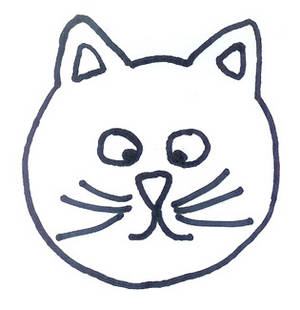
\includegraphics[height=0.8cm]{../img/cat.jpg}
}
\parbox{4.0cm}{
	Auch wichtig: Schrödingers Katze
}


% Ende der Spalten
\end{multicols}

% Dokumentende
% ======================================================================
\end{document}
